\documentclass[draft=True]{revtex4-2}
\newcommand{\zreco}{\ensuremath{\cos{(\theta_z^{reco})}}}
\newcommand{\ztrue}{\ensuremath{\cos{(\theta_z^{true})}}}
\newcommand{\emm}{\ensuremath{\epsilon_{\mu\mu}}}
\newcommand{\emt}{\ensuremath{\epsilon_{\mu\tau}}}
\newcommand{\eet}{\epsilon_{e\tau}}
\newcommand{\eem}{\epsilon_{e\mu}}
\newcommand{\ett}{\ensuremath{\epsilon_{\tau\tau}}}
\newcommand{\ep}{\ensuremath{\epsilon^\prime}}
\renewcommand{\ne}{\nu_e}
\newcommand{\Ereco}{E^{reco}}
\newcommand{\Etrue}{E^{true}}
\newcommand{\nm}{\nu_\mu}
\newcommand{\nt}{\nu_\tau}
\newcommand{\ane}{\bar\nu_e}
\newcommand{\anm}{\bar\nu_\mu}
\newcommand{\ant}{\bar\nu_\tau}
\newcommand{\dm}{\Delta m^2_{31}}
\newcommand{\sth}{\sin^2(2\theta_{23})}

\usepackage{physics,amsmath, amsfonts, siunitx, amssymb, graphicx, subcaption}
\usepackage[utf8]{inputenc}
\usepackage{hyperref}
\begin{document}
\section{Formalism of non-standard interactions}
Non-standard interactions are sub-leading contributions to neutrino flavor transitions arising from neutrino interactions not considered in the Standard Model.
We consider matter NSIs arising from the neutral current NSIs, which exclude production 
and detection effects. An effective four-fermion Lagrangian for this type of interaction can be written as
\begin{align}
   \mathcal{L}_{\mathrm{NC}} &= -2 \sqrt{2} G_{F} \epsilon_{\alpha \beta}^{f X}\left(\bar{\nu}_{\alpha} \gamma^{\mu} P_{L} \nu_{\beta}\right)\left(\bar{f} \gamma_{\mu} P_{X} f\right)\,,
\end{align}
where NC denotes the neutral current interaction with 
$f \in \{e,u,d\}$, and $P_X$ is the chirality projection operators with $X \in \{L,R\}$.  

For chirality $X$, the NSI Hamiltonian takes the form 
\begin{align}
   H &= \frac{1}{2E} UM^2U^\dagger + \sqrt{2}G_F n_e \text{diag}(1,0,0) + \sqrt{2}G_F \sum_f n_f \epsilon^{fX}
\end{align}

We have no independent sensitivity for the chirality of $\epsilon^{fX}$, so we sum over these to obtain the vectorial parameter as $\epsilon^{fV}_{\alpha\beta} = \epsilon^{fL}_{\alpha\beta}+ \epsilon^{fR}_{\alpha\beta}$.
Moreover, we normalize the fermion number density $n_f$ by
the electron number density $n_e$. Our matter study will be wholly confined to the interior of the Earth, where we assume electrical neutrality and equal distribution of neutrons and protons, 
so we use the relations $n_u/n_e \simeq n_d/n_e \simeq 3$.
The effective NSI parameters in matter now take the form
\begin{align} \label{eq:epsilon}
    \epsilon_{\alpha\beta} &= \sum_{f,X} \frac{n_f}{n_e} \epsilon^{fX}_{\alpha\beta} \nonumber \\
                           &= \epsilon_{\alpha\beta}^{eV} + 3\epsilon_{\alpha\beta}^{uV} + 3\epsilon_{\alpha\beta}^{dV}
\end{align}
We note that our definition of $\epsilon_{\alpha\beta}$ differs from some texts, where the quark number density is used to normalize
the parameters\cite{deepcoreNSI}.

With the matter potential $V = \sqrt{2}G_F n_e$, we write
\begin{align} \label{eq:H_NSI}
   H &= \frac{1}{2E} UM^2U^\dagger + V\,
   \begin{bmatrix}
      1 + \epsilon_{ee} & \epsilon_{e\mu} & \epsilon_{e\tau}  \\
      \epsilon_{e\mu} & \epsilon_{\mu\mu} & \epsilon_{\mu\tau}  \\
      \epsilon_{e \tau} & \epsilon_{\mu\tau} & \epsilon_{\tau\tau}
  \end{bmatrix}\,,
\end{align}
where we have assumed the components of the NSI matrix to be real. 

To propagate the neutrino states through the Earth, we solve the Schrödinger equation with the Hamiltonian from Eq.~\ref{eq:H_NSI}. 
The Earth density profile is taken from the PREM~\cite{PREM}. The baseline for a given trajectory is determined using an average neutrino
production height of 15 km and an Earth radius of 6371 km. The propagation does not include neutrino absorption. After this, we are
ready to study the NSI effect on probability level.
%TODO: add more here? are there more effects than just absoption missing? justify absorption missing?

\subsection{Non-standard effects in the GeV-TeV range}\label{sec:nsiEffects}
Since neutrinos and antineutrinos have different cross sections, they are treated separately in the detector simulations. 
However, for the purpose of qualitatively elucidating the NSI effect in this subsection, we take the effective area of $\nm$ and $\anm$ to be equal. 
Thus, we simply add the neutrino to the antineutrino contributions in both Fig.~\ref{fig:nsi_probs} and Fig.~\ref{fig:flux_ratio}.

In the $\mu\tau$ sector, we have a resonance in the \SI{20}{\GeV} region. Any NSI parameter involving the $\mu$ or $\tau$ channel will dampen this resonance,
with some also shifting the probability in the stationary region above \SI{100}{\GeV}.
This `double effect' of both resonance dampening and shifting happens in two cases: either when the NSI parameter shares one channel with a survival probability
(e.g. $\eem$ and $P_{\mu\mu}$), or when the sectors align (e.g. $\emt$ and $P_{\mu\tau}$). The only exception to this is for $P_{\tau\tau}$, 
which due to the near-maximal mixing in the $\mu\tau$ sector displays dampening for $\eem$ even though they share no channel directly. We illustrate
the three different effects in Fig.~\ref{fig:nsi_probs}. 

Due to the lightness of $\Delta m^2_{21}$, the $e$ channel has no resonance in the \si{\GeV} range. Thus, the only impact that 
the NSI parameters considered here can have on any $\nu_e$ probability is shifting, and this only occurs when the requirements for the `double effect'
are met. So except for the survival probability $P_{ee}$, any NSI parameter whose sector does not match the probability sector will not drastically affect it. 
Thus, the only off-diagonal NSI parameters that strongly affect the transition probabilities $P_{\alpha\beta}$ are $\epsilon_{\gamma\beta}$,
while the survival probabilities $P_{\alpha\alpha}$ are only strongly affected by $\epsilon_{\alpha\beta}$.
%TODO: make this clearer and give conclusion. Maybe also test for lower E around dm21 resonance. Add about realness and CP-invariance
\begin{figure}
   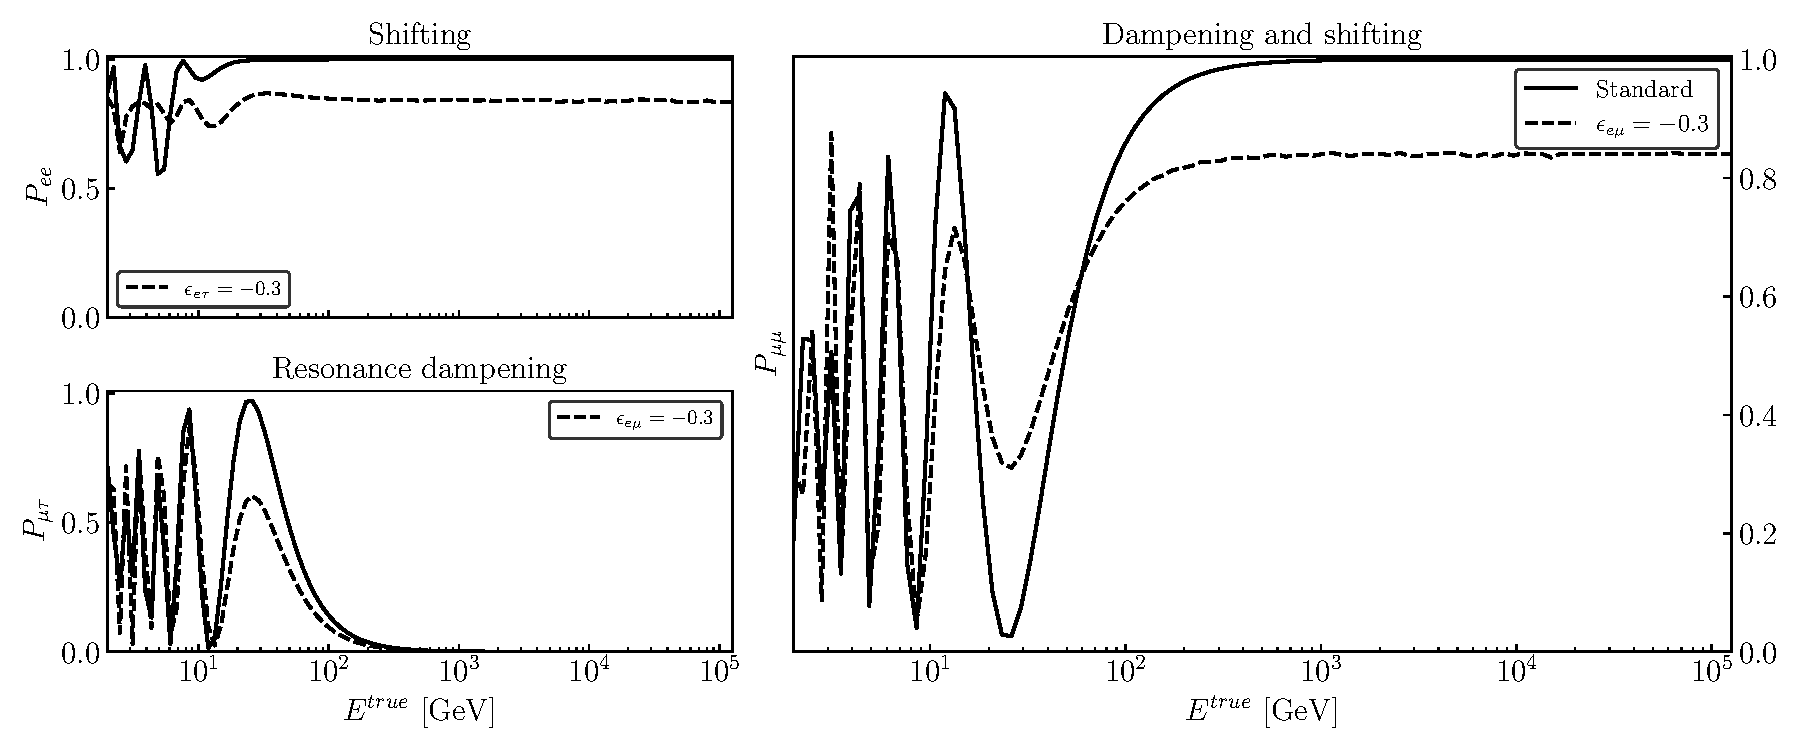
\includegraphics[width=0.95\textwidth]{figures/nsi_probs.pdf}
   \caption{The three different effects that the off-diagonal NSI parameters have in 
   the \si{\GeV} range. To schematically elucidate the NSI effect, we plot the summed probabilities for both neutrinos and 
   antineutrinos.}\label{fig:nsi_probs}
\end{figure}%TODO: change plot ylabels

To study the NSI flux effect, we propagate the atmospheric neutrino flux from Honda et al~\cite{hondapaper} through the Earth.
The oscillation probability $P_{\alpha \beta}$ acts as a weight to the atmospheric flux, yielding the propagated flux for flavor $\beta$ at detector level as 
\begin{align}\label{eq:propFlux}
    \phi_\beta^\text{det} = \sum_\alpha P_{\alpha\beta} \phi_\alpha^\text{atm} \,,
\end{align}
where we sum over the initial lepton flavors $\alpha \in \{e,\mu, \bar{e}, \bar{\mu}\}$. To illustrate the impact of $\emt$ at flux level, 
we plot in Fig.~\ref{fig:flux_ratio} the quantity $(\phi_{\nu_\mu}^{NSI} + \phi_{\bar\nu_\mu}^{NSI})/(\phi_{\nu_\mu}^{SI} + \phi_{\bar\nu_\mu}^{SI})$, 
where all fluxes are propagated to detector level by Eq.~\ref{eq:propFlux}. 
In the left panel, we plot the flux in region in which 99\% of the 
DeepCore track events originating from $\nm + \anm$ fluxes are contained. In the right panel, we show the same but with IceCube events. We see that the only clear signal discernible to the IceCube detector
is a energy-independent flux deficiency with a factor in the order of $\sim 10^{0.5}$ from core-crossing neutrinos within a zenith range of $\ztrue < -0.87$. DeepCore on the other hand, 
is exposed to multiple fringes of flux surpluses with a factor in the order of $\sim 10$. The strongest surplus at \SI{20}{\GeV} is very weakly zenith dependent, a stark contrast to the
energy-independent but zenith-sensitive IceCube deficiency.
%TODO: check values above after final plot of flux ratios

The muonic flux not only carries the largest $\emt$ effect, but it is also more abundant than the $\ne$ flux. Thus, we expect to receive the highest statistics from $\mu$-related NSI parameters,
thus constraining them the strongest. $\epsilon_{\alpha\beta}$ which are only indirectly weakly dependent on the $\mu$ channel will have the weakest bounds. This could be improved
by considering cascade events in IceCube, thus opening up the $e$ and $\tau$ channels there.

\begin{figure}[!tb]
   \begin{center}
      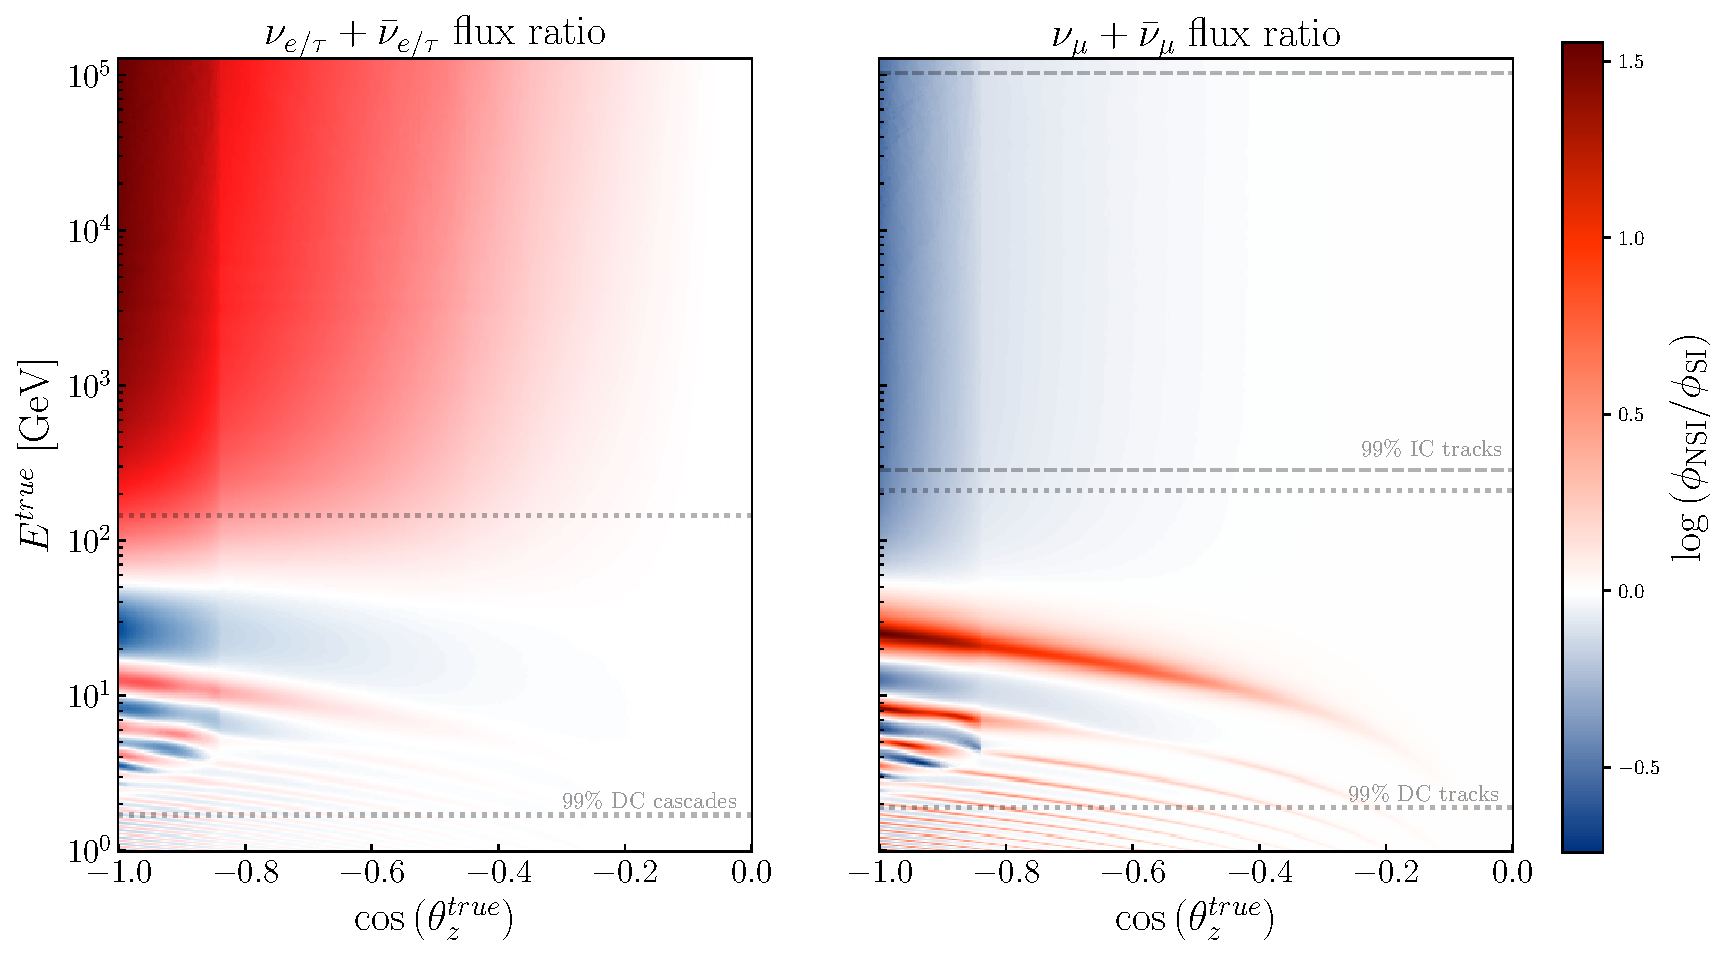
\includegraphics[width=0.8\linewidth]{figures/flux_ratio.pdf}
   \end{center}
   \caption{Ratio of detector NSI to SI atmospheric $\nu_\mu + \bar{\nu}_\mu$ fluxes expressed as $(\phi_{\nu_\mu}^{NSI} + \phi_{\bar\nu_\mu}^{NSI})/(\phi_{\nu_\mu}^{SI} + \phi_{\bar\nu_\mu}^{SI})$.
   We set $\emt = -0.05$, and all other $\epsilon_{\alpha\beta}=0$. 
   Left (right) panel shows the flux ratio in the energy range in which 99\% of the DeepCore (IceCube) events are contained.
   }\label{fig:flux_ratio}
\end{figure}%TODO: make prettier cmap 

\section{Detector formalism}
\subsection{IceCube}\label{ch:ICmethod}
We obtain the data from the IC-86 sterile data release~\cite{IC2020}, which was collected over 8 years. The event rate for each bin reads
\begin{align}\label{eq:ICevents}
   N_{ij} &= T\sum_\beta \int_{(\cos{\theta_z^r})_i}^{(\cos{\theta_z^r})_{i+1}} \dd \cos{\theta^r_z} \int_{E^r_{j}}^{E^r_{j+1}} \dd E^r \int_0^\pi R(\theta^r,\theta^t) \dd \cos{\theta^t} \int_0^\infty \phi_\beta^\text{det}(E^t,\theta^t)  A^\text{eff}(E^t) R(E^r,E^t) 
   \dd E^t\,,
\end{align}
where $T$ is the live time of the detector, and $A^\text{eff}$ its effective area averaged over the flavors $\beta$ from~\cite{ICaeff}. $R(x^r,x^t)$ is a resolution function, 
which is responsible for the smearing between the reconstructed and true parameters $x^r$ and $x^t$, respectively. We assume a log-normal distribution, giving it the form 
\begin{align}
    R(x^r, x^t) = \frac{1}{\sqrt{2\pi} \sigma_{x^r}x^r} \exp\left[-\frac{(\log x^r-\mu(x^t))^2}{2\sigma_{x^r}^2}\right]\,.
\end{align}
However, the energy reconstruction is biased, which means that we don't assume that $\mu(E^t) =E^r$~\cite{weaverEvidenceAstrophysicalMuon}. 
To model this relationship between $\Etrue$ and $\Ereco$, we train a Gaussian process regressor on the IC-86 Monte Carlo dataset from~\cite{IC2016}, from which
we can extract a predicted mean and standard deviation for a given $E^{reco}$. We then take the $\Etrue$ points of the 99th percentile of each distribution to obtain
the limits over which to integrate. We take the angular resolution function to be identically unity since the angle resolution in IceCube for track-like 
events is less than $\SI{2}{\degree}$, making $\ztrue$ practically coincide with $\zreco$ for our study~\cite{IC2020}. 

\subsection{DeepCore}\label{ch:DCmethod}
We use the publically available DeepCore data sample~\cite{DC2019data} which is an updated version of what was used by the 
IceCube collaboration in a $\nu_\mu$ disapprearance analysis~\cite{DC2018mudisappearance}.

The detector systematics include ice absorption and scattering, as well as overall, lateral, and head-on optical efficiencies of the DOMs. 
They are applied as correction factors using the best-fit points from the DeepCore 2019 $\nu_\tau$ appearance 
analysis~\cite{DC2019tauappearance}.

The data include 14901 track-like events and 26001 cascade-like events, both divided into eight 
$ \log_{10}E^{reco} \in [0.75,1.75]$ bins, and eight $\zreco \in [-1,1]$ bins. Each event has a Monte Carlo weight $w_{ijk,\beta}$
from which we can construct the event count as
\begin{align}\label{eq:MCevents}
    N_{ijk} &= C_{ijk}\sum_{\beta}w_{ijk,\beta}\, \phi_\beta^\text{det}\,,
\end{align}
where $C_{ijk}$ is the correction factor from the detector systematic uncertainty and $\phi_\beta^\text{det}$ is defined as Eq.~\ref{eq:propFlux}. We have now substituted the effect of the Gaussian smearing 
by treating the reconstructed and true quantities as a migration matrix. 

The oscillation parameters used on our DeepCore simulations are from the
best-fit in the global analysis in~\cite{nufit}: $\theta_{12} = \SI{33.44}{\degree},\, \theta_{13} = \SI{8.57}{\degree},\, \Delta m^2_{21} =  \SI{7.42}{\electronvolt^2}$, and we 
marginalize over $\dm$ and $\theta_{23}$ between their $3\sigma$ limits \SIrange{2.435e-3}{2.598e-3}{\eV \squared} and \SIrange{40.1}{51.7}{\degree}, respectively.

\subsection{PINGU}\label{ch:PINGUmethod}
The methodology behind the PINGU simulations is the same as with our DeepCore study~\ref{ch:DCmethod}. We use the public Monte Carlo~\cite{PINGUdata}, 
which allows us to construct the event count as in Eq.~\ref{eq:MCevents}.
However, since no detector systematics is yet modeled for PINGU, the correction factors $C_{ijk}$ are all unity. We will remedy this by including an uncorrelated systematic error.
As with the DeepCore Monte Carlo, the PINGU Monte Carlo is divided into eight 
$\log_{10}E^{reco} \in [0.75,1.75]$ bins, and eight $\zreco \in [-1,1]$ bins for both track- and cascade-like events. 
We plot the normalized event differences $(N_{NSI} - N_{SI})/\sqrt{N_{SI}}$ for cascades and tracks in Fig.~\ref{fig:event_pulls}. %TODO:talk about this
We generate `data' by predicting the event rates at PINGU with the following best-fit parameters from~\cite{nufit}, except for the CP-violating phase which is set to zero for simplicity.

\begin{align}\label{eq:PINGUparams}
    &\Delta m^2_{21} =  \SI{7.42e-5}{\electronvolt^2},\hspace{0.5em} \dm =  \SI{2.517e-3}{\electronvolt^2}, \nonumber \\
    &\theta_{12} = \SI{33.44}{\degree},\hspace{1em} \theta_{13} = \SI{8.57}{\degree},\hspace{1em} \theta_{23} = \SI{49.2}{\degree}, \hspace{1em} \delta_\text{CP} = 0\,.
\end{align}

\section{Results}
At the reconstructed event level, we note that the $\emt$ features discussed in Sec.~\ref{sec:nsiEffects} display themselves differently in each detector.
We investigate this for $\emt$ by in Fig.~\ref{fig:Pmm_asymmetry} plotting the muon survival probability difference $P_{\mu\mu}(\epsilon^+_{\mu\tau}) - P_{\mu\mu}(\epsilon^-_{\mu\tau})$, where 
%TODO: check that this is what is plotted.
$\epsilon^\pm_{\mu\tau} = \pm 0.01$.
Comparing Fig.~\ref{fig:Pmm_asymmetry} with the flux ratios in Fig.~\ref{fig:emt_events}, we see that the reconstruction of PINGU is
superior to DeepCore, since the event ratio $\log{(N^+_{NSI}/N^-_{NSI})} = \log{N^+_{NSI}} - \log{N^-_{NSI}}$ (in reconstructed quantities) 
more closely matches the probability difference $P^+-P^-$ (in true quantities).
This is most evident below \SI{20}{\GeV}, where the DeepCore reconstruction has washed out the fringes while PINGU preserves the $N^-_{NSI}$ surplus below \SI{10}{\GeV}.

Now we turn to the effect of $\emt$. Muon events are the most abundant, and it suffices to study $P_{\mu\mu}$ in this way to explain the $\emt$ features. 
First, let $P^\pm$ denote $P_{\mu\mu}(\epsilon^\pm_{\mu\tau})$. 
We see see that $\emt^+$ generates a slightly higher $P_{\mu\mu}$ for energies around \SI{20}{\GeV} (blue area),
while $\emt^-$ produces higher $P_{\mu\mu}$ for almost all other combinations of ${\Etrue,\ztrue}$. As we see in Fig.~\ref{fig:flux_ratio}, this muon survival abundance 
is indeed preserved at flux level. So the flux for $\emt^+$ is higher than the flux for $\emt^-$. Is this still true at event level, i.e. after reconstruction? 
As we see in Fig.~\ref{fig:emt_events}, the binned PINGU event counts display strong differences for many bins, which will give a high statistics on both sides of $\emt=0$, slightly favoring $\emt^-$. 
DeepCore on the other hand, has fewer bins where the event count for $\emt^-$ surpasses the event count for $\emt^+$, 
giving weaker statistics for the negative side. Thus, we conclude that we will see a $\emt$ \si{GeV}-asymmetry stemming from the lower statistics 
for negative $\emt$ at probability level, which is then propagated through the flux and finally affects the reconstruction. %TODO: fill more conclusion?

\begin{figure}
   \begin{subfigure}{0.25\textwidth}   
      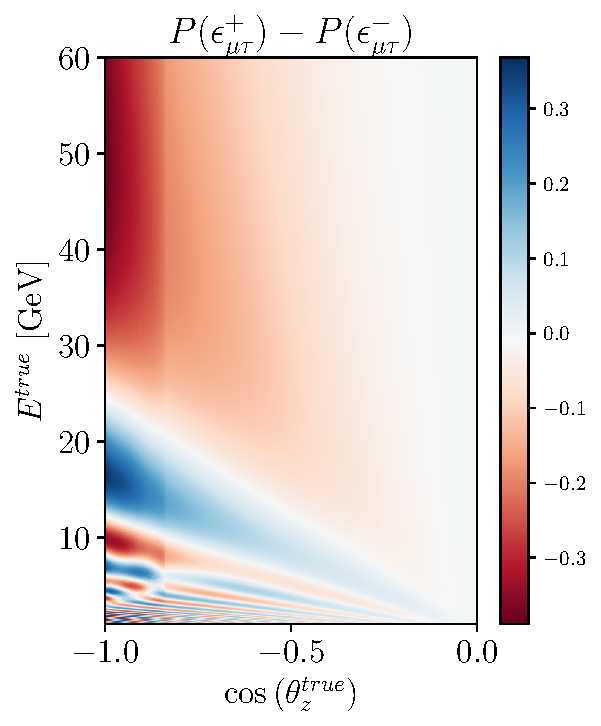
\includegraphics[width=1\linewidth]{figures/Pmm_asymmetry.pdf}%TODO: redo for emt=0.01x
      \caption{$P_{\mu\mu}(\epsilon^+_{\mu\tau}) - P_{\mu\mu}(\epsilon^-_{\mu\tau})$ using  $\epsilon^\pm_{\mu\tau} = \pm 0.01$}\label{fig:Pmm_asymmetry}
   \end{subfigure}
   \begin{subfigure}{0.6\textwidth}
      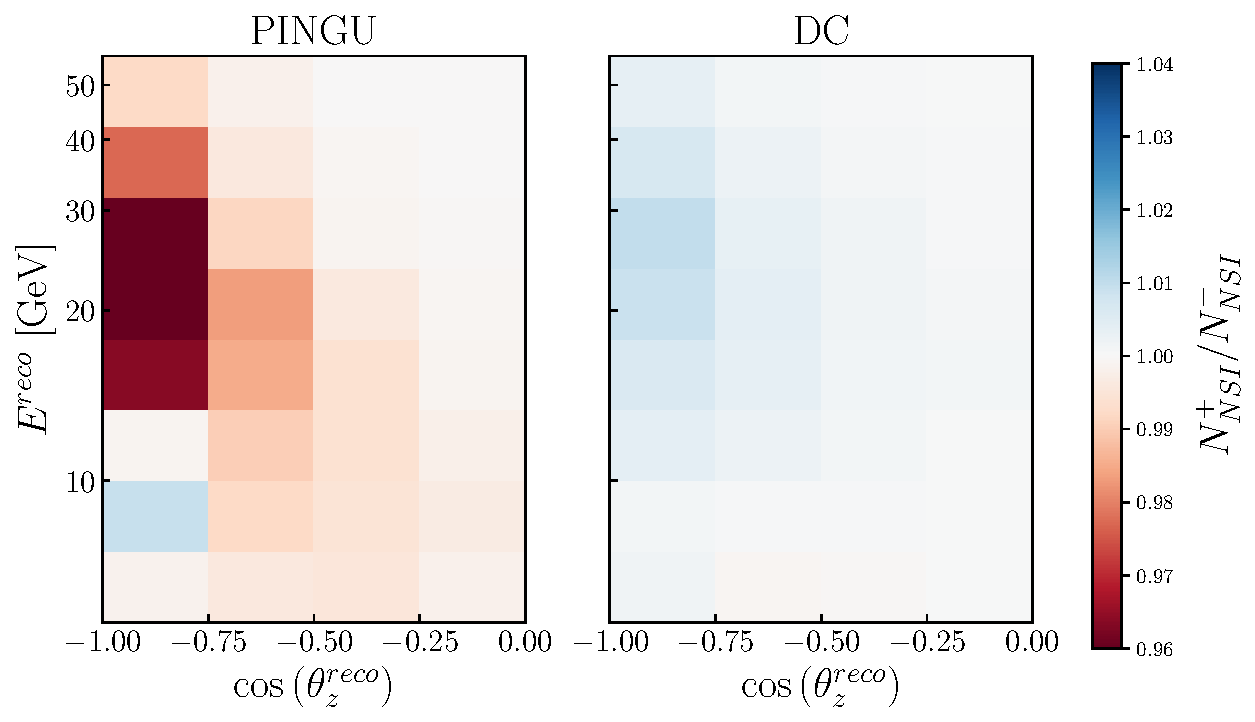
\includegraphics[width=1\linewidth]{figures/emt_events.pdf}
   \caption{The best-fit event count ratio from each detector for $\emt = \pm 0.01$. IceCube only observes a small surplus of events for $\emt=-0.01$ compared to 
   DeepCore and PINGU due to the weak NSI effect at high \si{\GeV} energies.}\label{fig:emt_events}%TODO: improve caption?
   \end{subfigure}
   \caption{Probability difference and best-fit event count. Negative $\emt$ has the strongest signal, as the thin blue 
   region stemming from $\emt = 0.01$ is less prominent than the red regions from $\emt=-0.01$.}
\end{figure}
 
\subsection{Constraining the NSI parameters}\label{sec:method}
In this section, we will constrain the four NSI parameters $\ett$, $\emt$, $\eem$, and $\eet$ by considering the detectors separately as well as jointly.
For our analyses, we define our $\chi^2$ as
\begin{align} \label{eq:chisq}
    \chi^{2}(\hat{\theta},\alpha,\beta, \kappa)=\sum_{ijk} \frac{\left(N^\text{th}-N^\text{data}\right)_{ijk}^{2}}
    {\left(\sigma^\text{data}_{ijk}\right)^{2} + \left(\sigma^\text{syst}_{ijk}\right)^{2}}+ 
    \frac{(1-\alpha)^2}{\sigma_\alpha^2} + \frac{\beta^2}{\sigma_\beta^2}\,
\end{align}
where we minimize over the model parameters $\hat{\theta} \in \{\dm, \theta_{23}, \epsilon\}$, the penalty terms $\alpha$ and $\beta$, and the free parameter $\kappa$.
$N_{ijk}^\text{th}$ is the expected number of events from theory, and $N_{ijk}^\text{data}$ is the observed number of events in that bin. 
We set $\sigma_\alpha = 0.25$ as the atmospheric flux normalization error, and $\sigma_\beta = 0.04$ as the zenith angle slope error~\cite{hondapaper}. 
The observed event number has an associated Poissonian uncertainty $\sigma_{ijk}^\text{data} = \sqrt{N_{ijk}^\text{data}}$.
For IceCube, the event count takes the form
\begin{align}
    N^\text{th}_{ijk} = \alpha\left[1+\beta (0.5 + \zreco_i )\right] N_{ijk}(\hat{\theta})\,,
\end{align}
with $N_{ijk}(\hat{\theta})$ from Eq.~\ref{eq:ICevents}. Here, we allow the event distribution to rotate around the median zenith angle of $\zreco = -0.5$.

For DeepCore and PINGU, and the event count takes the form
\begin{align}
    N^\text{th}_{ijk} = \alpha\left[1+\beta \zreco_i \right] N_{ijk}(\hat{\theta}) + \kappa N_{ijk}^{\mu_{atm}}\,,
\end{align}
with $N_{ijk}(\hat{\theta})$ from Eq.~\ref{eq:MCevents}. $N_{ijk}^{\mu_{atm}}$ is the muon background, which is left to float freely in the DeepCore analysis.
The background at PINGU can be considered negligible to first order~\cite{PINGUdata}, and we thus put $\kappa=0$ when calculating the PINGU $\chi^2$.
For DeepCore and PINGU, the median zenith angle is $\zreco = 0$, we allow the event count to rotate around this point.

We treat the uncorrelated systematic uncertanties differently for each detector. For IceCube, we set $\sigma_{ijk}^\text{syst} = f\sqrt{N_{ijk}^\text{data}}$.
We consider best, normal, and worst-case scenarios in IceCube using
$f=5\%$, $10\%$, and $15\%$ respectively. For PINGU, we use the same form but instead use $f=0\%$, $3\%$, and $5\%$. %TODO: maybe source/justification for these values?
For DeepCore, we use the provided systematic error distribution which accounts for uncertainties in the finite MC statistics and the data-driven 
muon background estimate~\cite{DC2019data}. This is summarized in Table~\ref{table:syst_errors}.  %TODO segue
{\renewcommand{\arraystretch}{1.2}
\begin{table}
   \begin{tabular}{lccc}
      \hline \hline
      Experiment & Best case & Baseline & Worst case \\
      \hline
      IceCube & $5\%$ & $10\%$ & $15\%$ \\
      PINGU & $0\%$ & $3\%$ & $5\%$ \\
      \hline \hline
   \end{tabular}
   \caption{Definition of the best, baseline, and worst case scenarios considered in each experiment, modelled by $\sigma_{ijk}^\text{syst} = f\sqrt{N_{ijk}^\text{data}}$ with $f$ from the table.
   We do not consider different DeepCore scenarios because her systematic error distribution is already provided in the data release~\cite{DC2019data}.}\label{table:syst_errors}
\end{table}

For the joint analysis, we follow the parameter goodness-of-fit prescription~\cite{maltoni2003} and construct the joint $\chi^2$ as 
\begin{align}\label{eq:joint_chisq}
    \chi^2_\text{joint} = \sum_\text{exp}\chi^2_\text{exp} - \chi^2_\text{exp,min}\,
\end{align}
with test statistic $\chi^2_\text{joint,min}$. The $\Delta \chi^2_\text{joint}$ is then $\Delta \chi^2_\text{joint} = \chi^2_\text{joint} - \chi^2_\text{joint,min}$.

Now, we set all standard oscillation parameters to their current best-fit values of Eq.~\ref{eq:PINGUparams}, except for $\dm$ and $\theta_{23}$, 
which we marginalize over their $3\sigma$ ranges of \SI{2.435e-3} to \SI{2.598e-3}{\electronvolt^2} and \SI{40.1} to \SI{51.7}{\degree} respectively. %TODO: make unit ranges nicer.
After the oscillation parameters have been marginalized out, we plot $\Delta \chi^2$ for each of the four NSI parameters in Fig.~\ref{fig:3D_NO}. The results are shown in Fig.~\ref{fig:IC_3D} and summarized in Tables~\ref{table:IC_DC_results} and~\ref{table:PINGU_joint_results}.

Comparing the PINGU and the DeepCore results in Fig.~\ref{fig:3D_NO}, we note that the best-fit for each NSI parameter for the PINGU experiment is expected to be zero. This is because the `data' we generated during 
the PINGU simulations assume no NSI since they have yet to be observed in nature. This introduces a non-NSI bias in all joint analyses which include PINGU,
since PINGU has stronger statistics than DeepCore and will thus pull the joint $\chi^2$ towards $\epsilon =0$.

\begin{figure}
   \begin{center}
      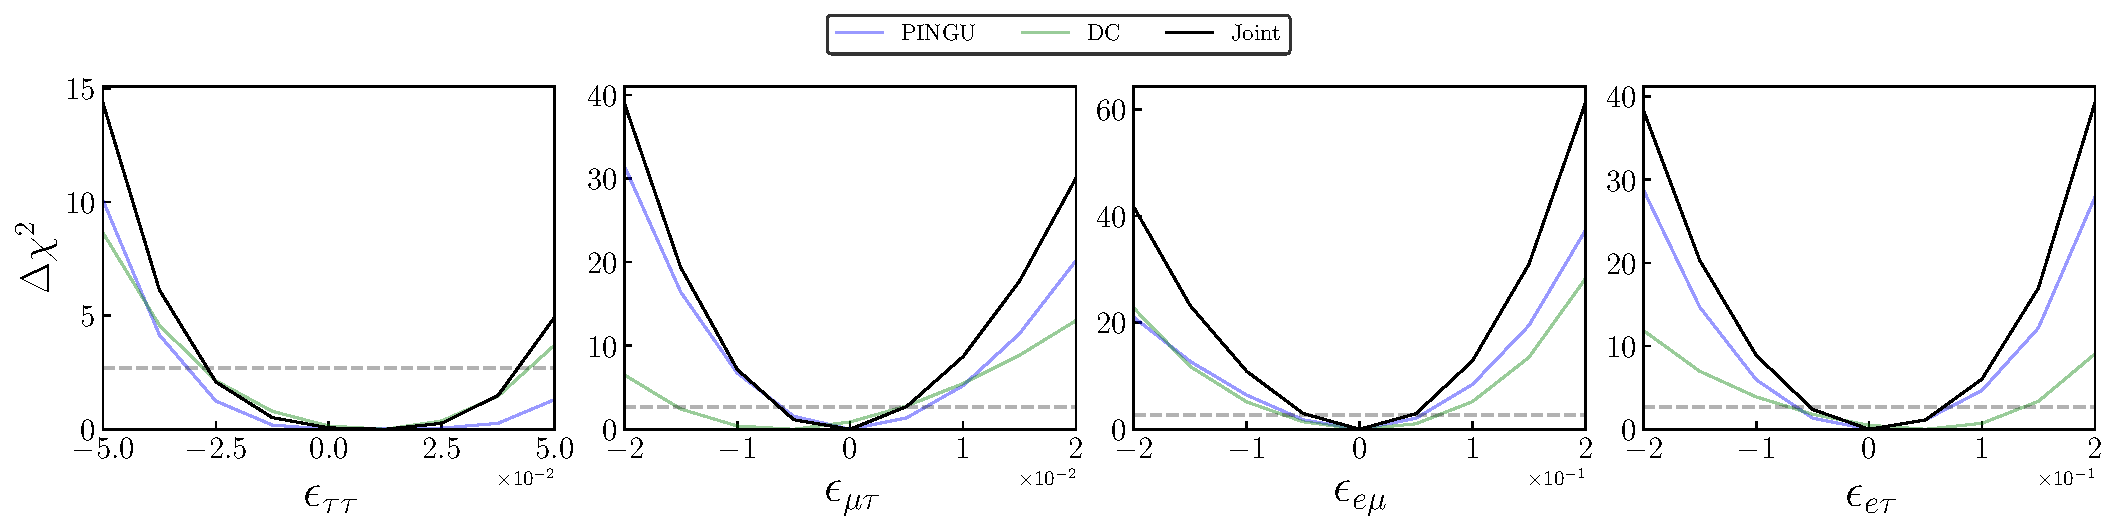
\includegraphics[width=0.6\textwidth]{figures/joint_3D_NO.pdf}
      \caption{PINGU and DeepCore best-case scenario, with their joint $\Delta \chi^2$ in black. $\dm$ and $\theta_{23}$ and have been marginalized out, and all other NSI 
      parameters not shown in each panel are fixed to zero. 
      IceCube tracks only reveal $\emt$, and are displayed separately in Fig.~\ref{fig:IC_3D}.}\label{fig:3D_NO}
   \end{center}
\end{figure} 
\begin{figure}
   \begin{center} 
      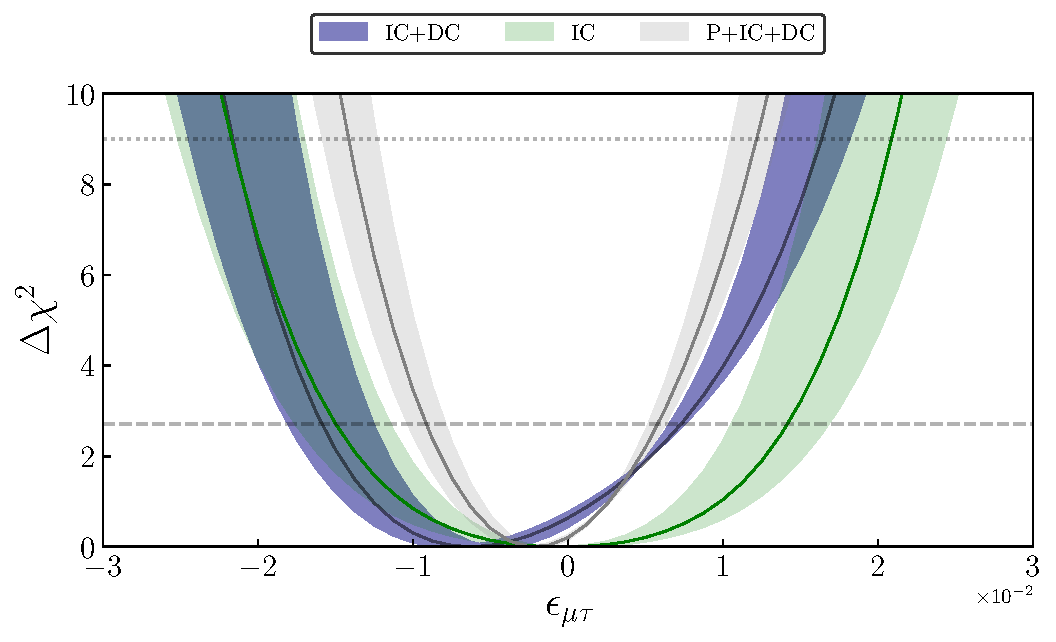
\includegraphics[width=0.6\textwidth]{figures/PID_3D_emt.pdf}
      \caption{$\emt$ $\Delta \chi^2$ regions for scenarios as defined in Table~\ref{table:syst_errors}.
    $\dm$ and $\theta_{23}$ and have been marginalized out, and all other NSI 
    parameters other than $\emt$ are fixed to zero.}\label{fig:IC_3D}
   \end{center}
\end{figure}



{\renewcommand{\arraystretch}{1.3}
 \begin{table}
   \begin{center}
   \begin{tabular}{lcccccc}
      \hline \hline
      Parameter & Best 90\% CL & Best $3\sigma$& Baseline 90\% CL & Baseline $3\sigma$ & Worst 90\% CL & Worst $3\sigma$\\
      \hline & \multicolumn{6}{c}{IceCube}  \\
      $\emt$ &  [-0.008, 0.009] &  [-0.014, 0.017] &   [-0.009, 0.01] &  [-0.015, 0.018] &   [-0.01, 0.011] &   [-0.017, 0.02] \\\\
      & \multicolumn{6}{c}{DeepCore}\\ [0.3em]
      $\ett$ &  [-0.044, 0.051] &  [-0.062, 0.069] &  [-0.046, 0.054] &         [-0.065] &  [-0.049, 0.057] &          [-0.07] \\
      $\emt$ &  [-0.008, 0.009] &  [-0.014, 0.017] &   [-0.009, 0.01] &  [-0.015, 0.018] &   [-0.01, 0.011] &   [-0.017, 0.02] \\
      $\eem$ &  [-0.079, 0.081] &   [-0.16, 0.14] &  [-0.11, 0.094] &  [-0.20, 0.16] &   [-0.14, 0.11] &   [-0.23, 0.18] \\
      $\eet$ &  [-0.079, 0.098] &  [-0.15, 0.16] &   [-0.10, 0.11] &  [-0.19, 0.18] &  [-0.13, 0.13] &  [-0.23, 0.12] \\\\
      &\multicolumn{6}{c}{IceCube + DeepCore}\\
      $\emt$ &  [-0.029, 0.007] &          [0.026] &  [-0.029, 0.007] &          [0.026] &  [-0.029, 0.007] &          [0.026] \\
      \hline
      \hline
   \end{tabular}
   \end{center}
   \caption{IceCube and DeepCore results from the $\Delta \chi^2$ in Fig.~\ref{fig:IC_3D}. Best, baseline, and worst refer to 
   the systematic uncertainty scenarios considered as in Table~\ref{table:syst_errors}.}\label{table:IC_DC_results}
\end{table}
\begin{table}
   \begin{tabular}{lcccccc}
      \hline \hline
      Parameter & Best 90\% CL & Best $3\sigma$& Baseline 90\% CL & Baseline $3\sigma$ & Worst 90\% CL & Worst $3\sigma$\\
      \hline & \multicolumn{6}{c}{PINGU} \\
      $\ett$ &  [-0.054, 0.067] &               [] &  [-0.054, 0.067] &               [] &  [-0.054, 0.067] &               [] \\
      $\emt$ &  [-0.029, 0.007] &          [0.026] &  [-0.029, 0.007] &          [0.026] &  [-0.029, 0.007] &          [0.026] \\
      $\eem$ &  [-0.12, 0.15] &  [-0.23, 0.24] &  [-0.12, 0.15] &  [-0.23, 0.24] &  [-0.12, 0.15] &  [-0.23, 0.24] \\
      $\eet$ &   [-0.084, 0.15] &  [-0.19, 0.21] &   [-0.084, 0.15] &  [-0.19, 0.21] &   [-0.084, 0.15] &  [-0.19, 0.21] \\\\
      & \multicolumn{6}{c}{DeepCore + PINGU} \\
      $\ett$ &  [-0.036, 0.046] &  [-0.056, 0.064] &  [-0.038, 0.048] &  [-0.058, 0.067] &   [-0.039, 0.05] &          [-0.06] \\
      $\emt$ &  [-0.009, 0.006] &  [-0.015, 0.013] &   [-0.01, 0.006] &  [-0.016, 0.014] &  [-0.011, 0.007] &  [-0.017, 0.015] \\
      $\eem$ &   [-0.06, 0.077] &  [-0.126, 0.127] &  [-0.071, 0.086] &  [-0.149, 0.141] &  [-0.082, 0.097] &  [-0.17, 0.16] \\
      $\eet$ &  [-0.052, 0.095] &  [-0.112, 0.144] &  [-0.061, 0.103] &  [-0.131, 0.155] &  [-0.067, 0.11] &  [-0.15, 0.17] \\\\
      & \multicolumn{6}{c}{IceCube + DeepCore + PINGU}  \\
      $\emt$ &  [-0.009, 0.006] &  [-0.015, 0.013] &   [-0.01, 0.006] &  [-0.016, 0.014] &  [-0.011, 0.007] &  [-0.017, 0.015] \\
      \hline
      \hline
   \end{tabular}
   \caption{PINGU and joint results from the $\Delta \chi^2$ in Fig.~\ref{fig:3D_NO}. Best, baseline, and worst refer to 
   the systematic uncertainty scenarios considered as in Table~\ref{table:syst_errors}.}\label{table:PINGU_joint_results}
\end{table}

\begin{table}
   \begin{center}
   \begin{tabular}{lccc}
           \hline \hline & \multicolumn{3}{c} {\text {Best fit}} \\
           \cline { 2 - 4 } Parameter & $\dm$ & $\theta_{23}$  & $\epsilon$  \\
           \hline \multicolumn{3}{c} {\hspace{2.5cm} DeepCore }  \\[0.1em]
           $\ett$ &  2.435 & 47.84 & 0.0125 \\
           $\emt$ &  2.435 & 43.97 & -0.005 \\
           $\eem$ &  2.435 & 43.97 & 0 \\
           $\eet$ &  2.435 & 43.97  & 0.05 \\\\
           \multicolumn{3}{c} {\hspace{2.5cm} IceCube } \\
           $\emt$ &  2.435 & 51.70 & 0 \\
           \multicolumn{3}{c} {\hspace{2.5cm} IceCube + DeepCore } \\
           $\emt$ &  2.517 & 43.97 & -0.01 \\
           \hline
           \hline
   \end{tabular}
   \end{center}
   \caption{Best fit points for $\dm$ and $\theta_{23}$ are given in units of $\si{10^{-3}\eV\squared}$ and
   degrees, respectively.}\label{table:bestfit}
\end{table}
\newpage


 \begin{figure}[t]
   \begin{center}
      \begin{subfigure}{0.38\textwidth}
         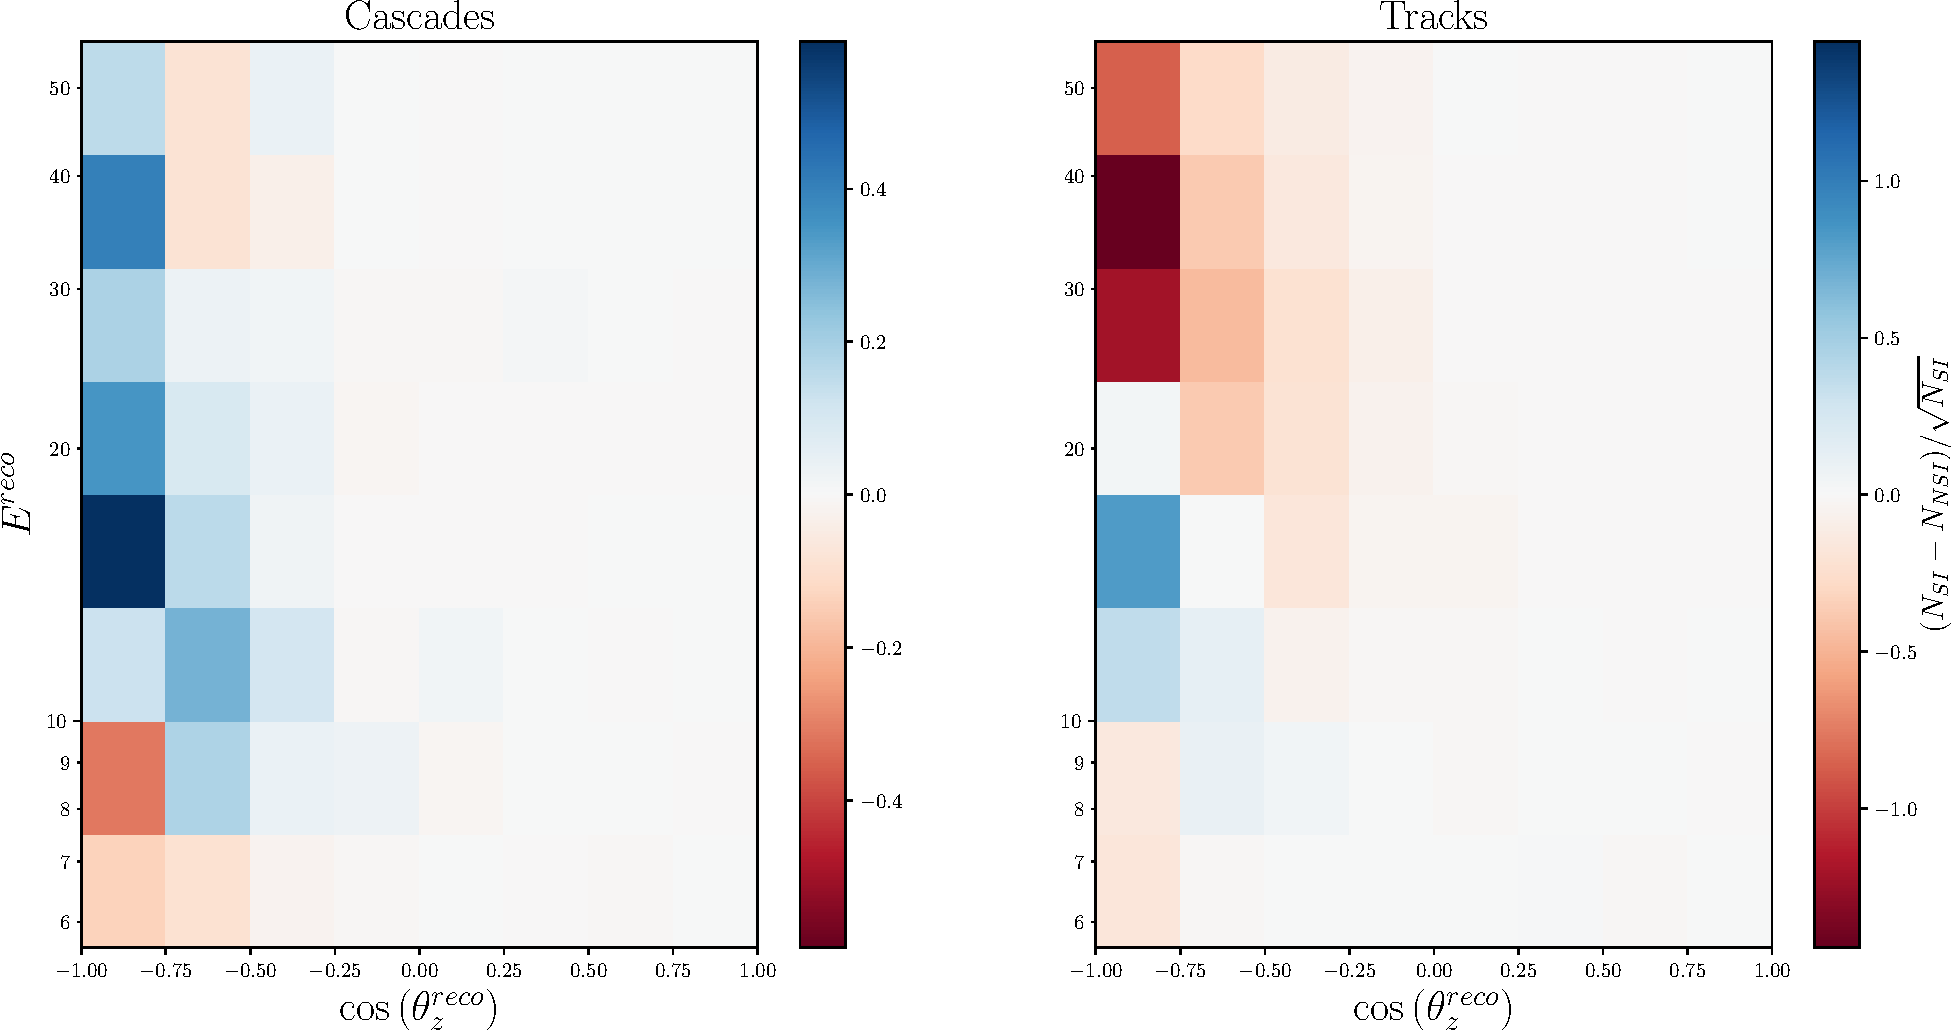
\includegraphics[width=1\linewidth]{figures/PINGU_event_pulls.pdf}
         \caption{PINGU}\label{fig:PINGU_event_pulls}
      \end{subfigure}
      \begin{subfigure}{0.4\textwidth}
         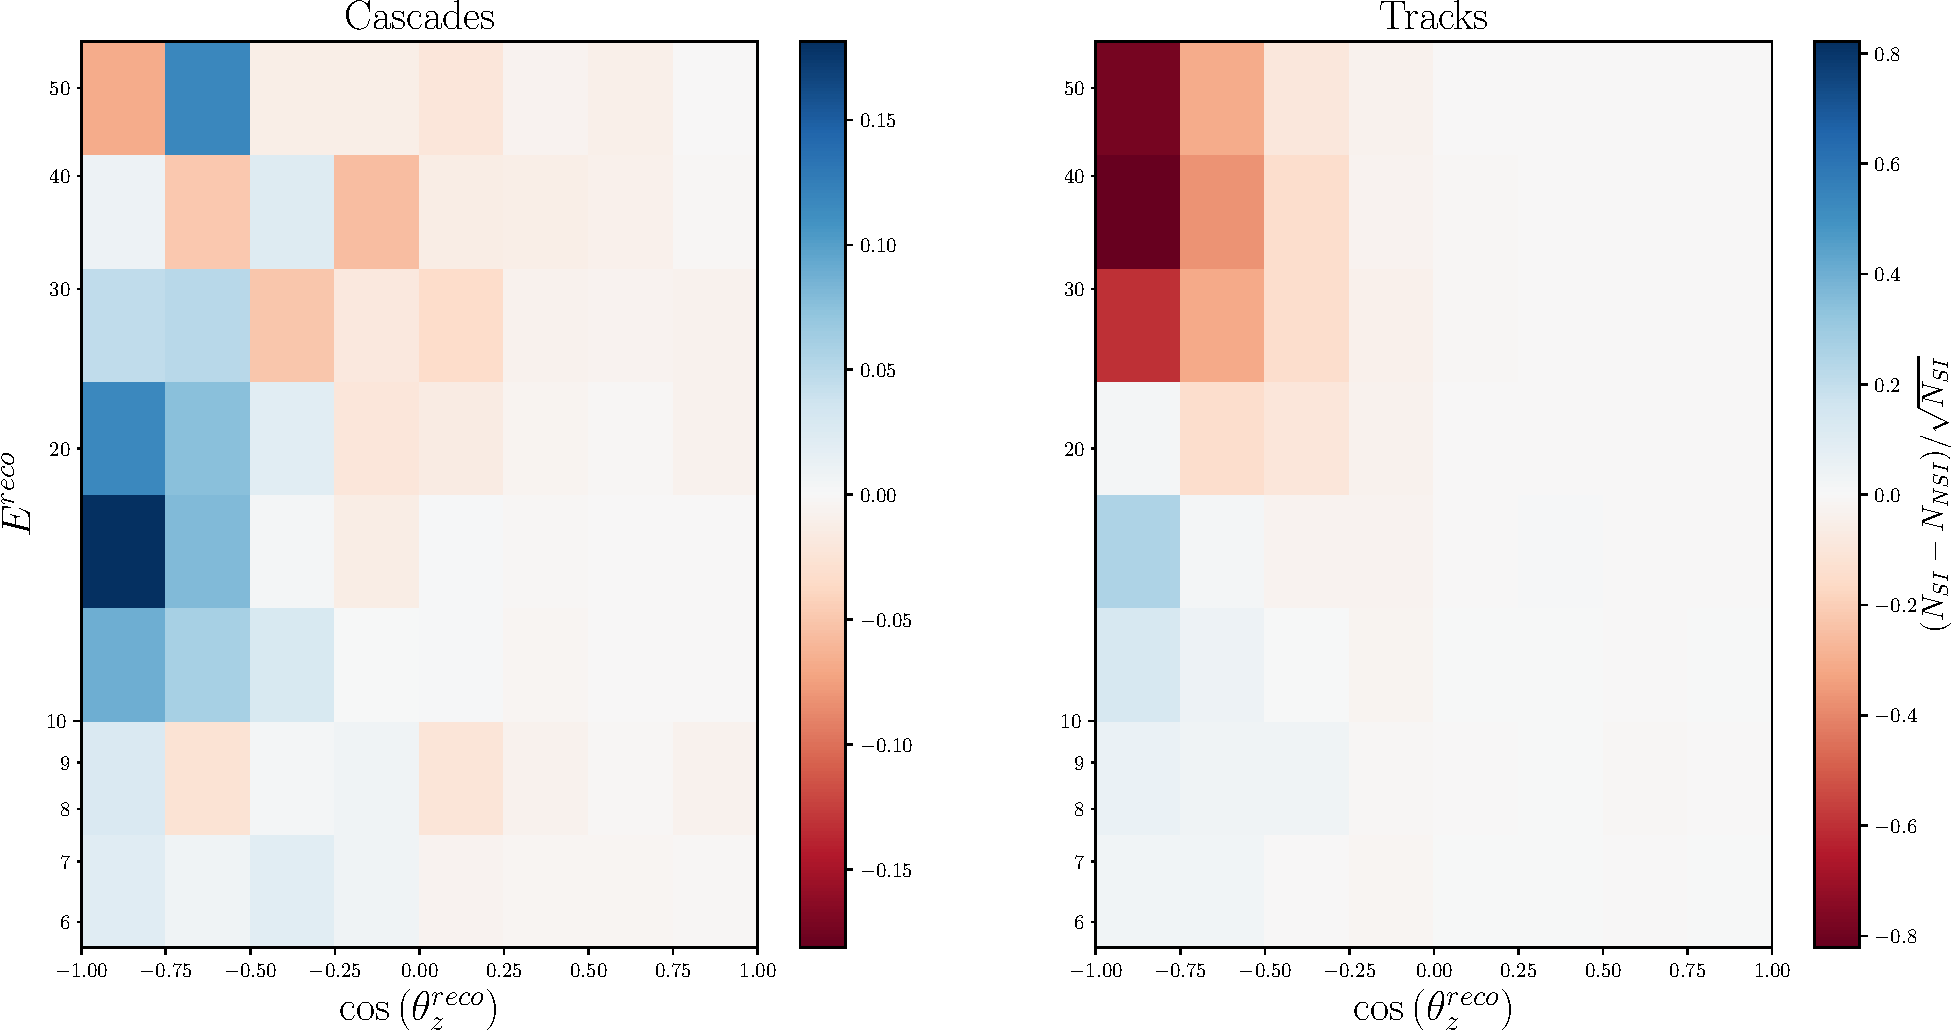
\includegraphics[width=1\linewidth]{figures/DC_event_pulls.pdf}
         \caption{DeepCore}\label{fig:DC_event_pulls}
      \end{subfigure}
    \end{center}
   \caption{Expected pulls of the form $(N_{NSI} - N_{SI})/\sqrt{N_{SI}}$ for PINGU and DeepCore after 3 years.}\label{fig:event_pulls} 
\end{figure}%TODO: redo these with same emt as flux_ratio? keep this, but align them better



%TODO: subsection about comparison between different papers. 

\begin{figure}
   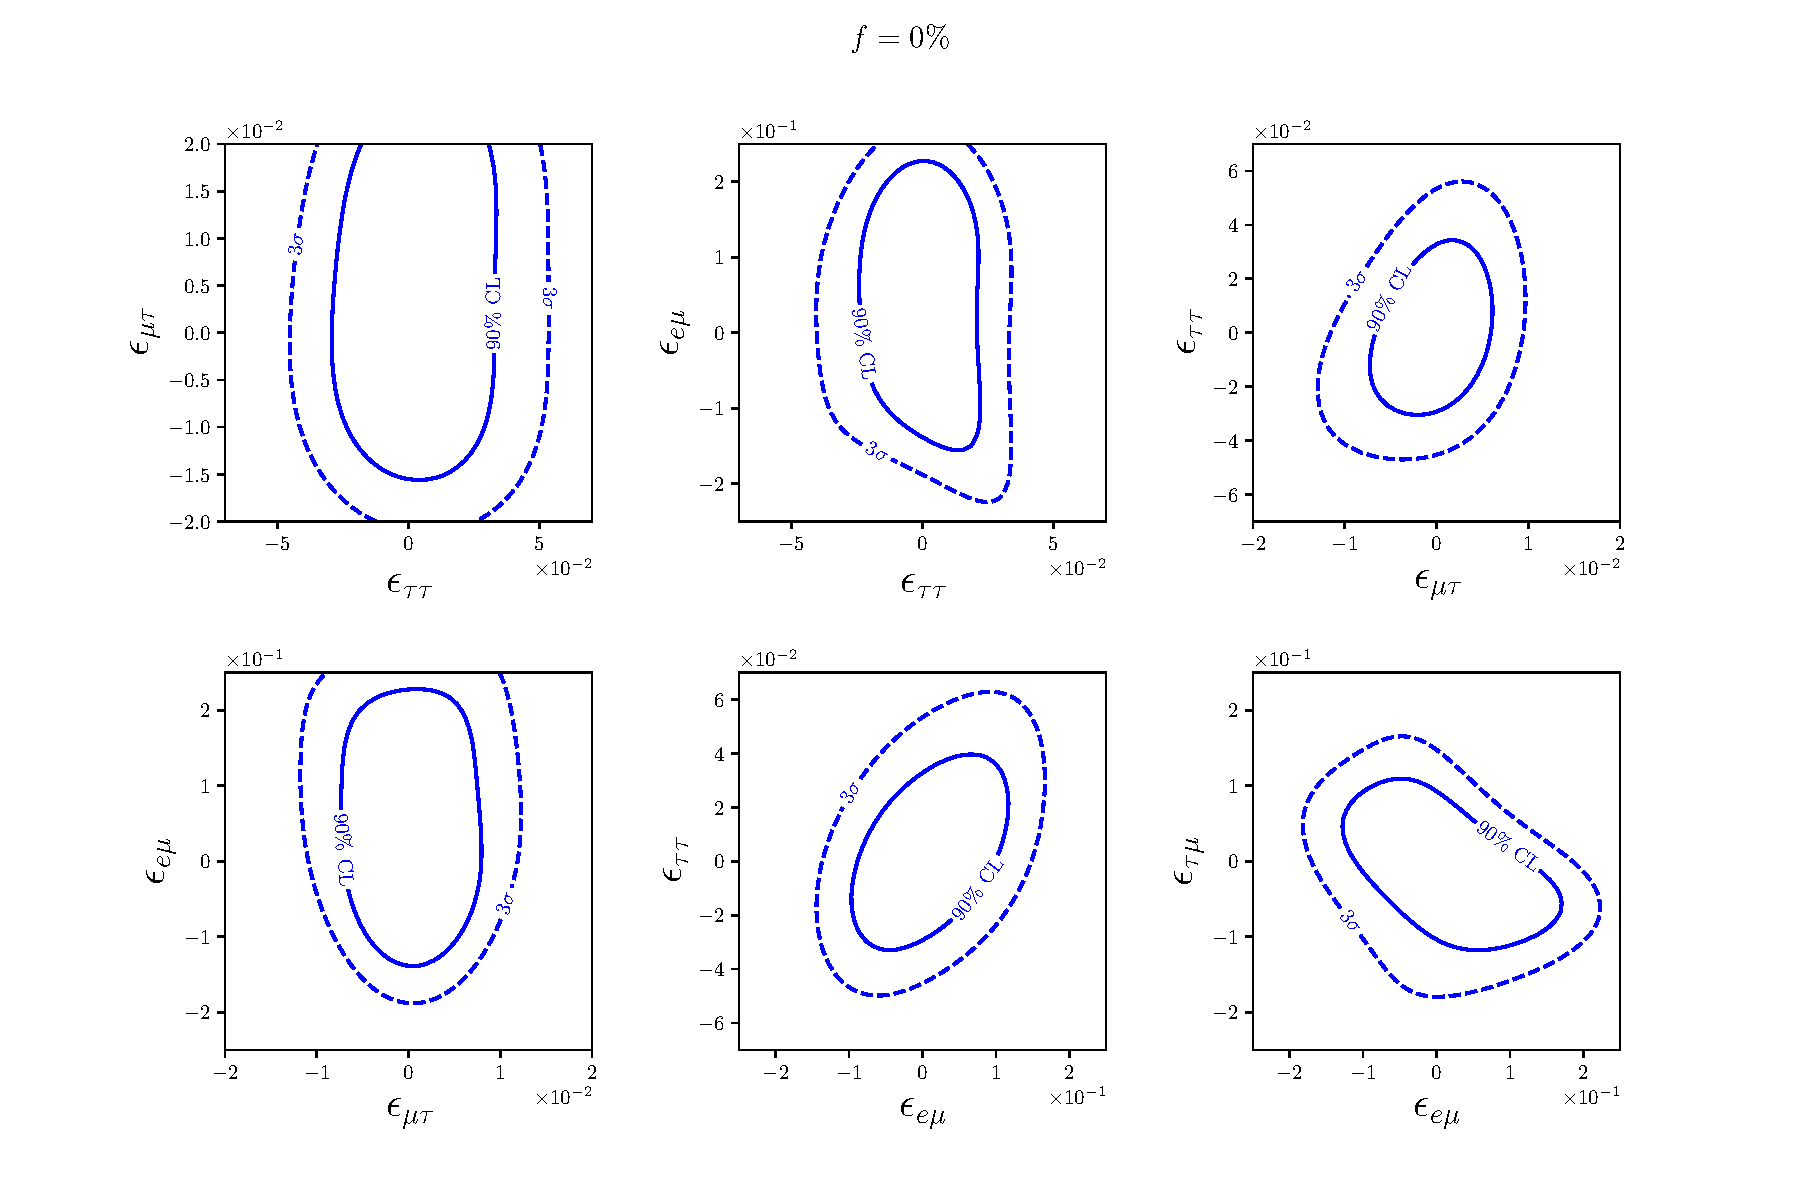
\includegraphics[width=0.9\textwidth]{figures/PINGU_2D_all_f0.pdf}
\end{figure}
\begin{figure}
   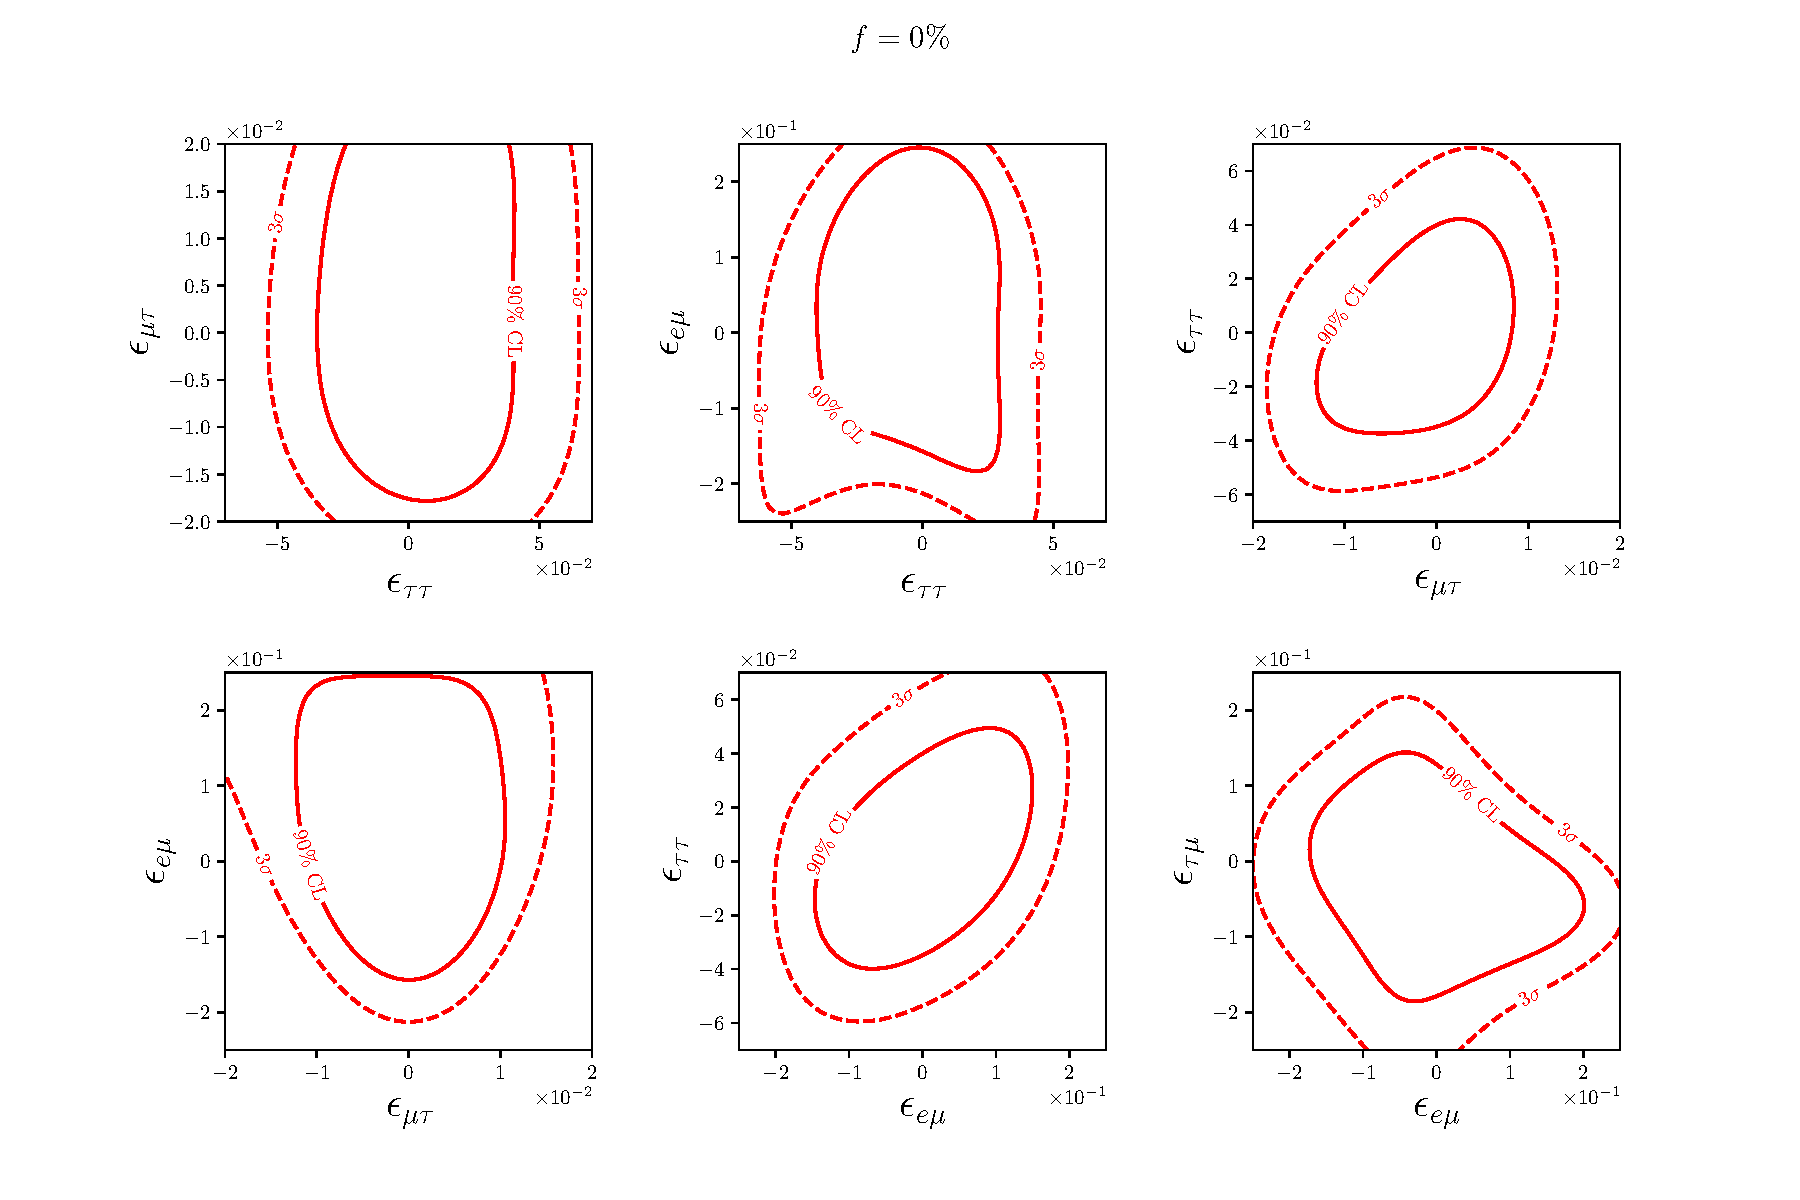
\includegraphics[width=0.9\textwidth]{figures/PINGU_2D_all_f5.pdf}
\end{figure}
\bibliographystyle{elsarticle-num}
\bibliography{article}

\newpage
\begin{tabular}{p{55mm}p{55mm}p{55mm}}
   DeepCore (2017)
      \begin{itemize}
         \item[$\checkmark$] Honda atmospheric fluxes
         \item[$\times$] Only look at tracks and $\emt$
         \vspace{1em}  
         \item[$\times$] DC Monte Carlo from an older dataset 
         \item[$\times$] 8 E bins from $\SI{6.3}{\electronvolt^2}$ to $\SI{56}{\electronvolt^2}$
         \item[$\times$] 8 z bins from -1 to 0 
         \item[$\times$] Use "Overall" and "relative $\ne$ to $\nm$" normalization
         \item[$\times$] Prior on spectral index
         \item[$\times$] No zenith angle normalization
         \item[$\checkmark$] No priors on $\dm, \theta_{23},\theta_{13}$
      \end{itemize} &
    Demidov (2020) DC analysis
      \begin{itemize}
         \item[$\checkmark$] Honda atmospheric fluxes
         \item[$\checkmark$] Looks at tracks + cascades for $\emt$ and $\ett$
         \item[$\checkmark$] Data and Monte Carlo from DC 2018
         \item[$\checkmark$] 8 E bins from $\SI{5.6}{\electronvolt^2}   $ to $\SI{56}{\electronvolt^2}$
         \item[$\checkmark$] 8 z bins from -1 to 1
         \item[$\times$] Use "Overall" and "relative $\ne$ to $\nm$" normalization
         \item[$\times$] Prior on spectral index
         \item[$\times$] No zenith angle normalization
         \item[$\checkmark$] No priors on $\dm, \theta_{23}$
         \item[$\checkmark$] Fixes $\Delta m^2_{21}, \theta_{12}, \theta_{13}$
         \item[$\times$] Uncertainty on hadron production in atmosphere
         \item[$\times$] Uncertainty on neutrino nucleon cross section 
      \end{itemize} &
    This DC+PINGU analysis
      \begin{itemize}
         \item[$\checkmark$] Honda atmospheric fluxes
         \item[$\checkmark$] Tracks and cascades for all flavors
         \vspace{1em} 
         \item[$\checkmark$] Reco $\to$ true mapping from Monte Carlo migration matrix
         \item[$\checkmark$] 8 E bins from $\SI{5.6}{\electronvolt^2}$ to $\SI{56}{\electronvolt^2}$
         \item[$\checkmark$] 8 zenith angle bins from -1 to 1
         \item[$\checkmark$] Flux normalization uncertainty of 25\%
         \item[$\checkmark$] Zenith angle uncertainty of 4\% 
         \item[$\checkmark$] No priors on oscillation parameters 
         \item[$\checkmark$] Marginalize $\dm$ and $\theta_{23}$. All other oscillation parameters are fixed.
      \end{itemize} 
\end{tabular}
\end{document}


